
\begin{enumerate}
\item The function $f$ is plotted at Figure~\ref{fig:fctf}. This figure
gives us the intuition that the function is convex. 


  \begin{figure}[htb]
    \begin{center}
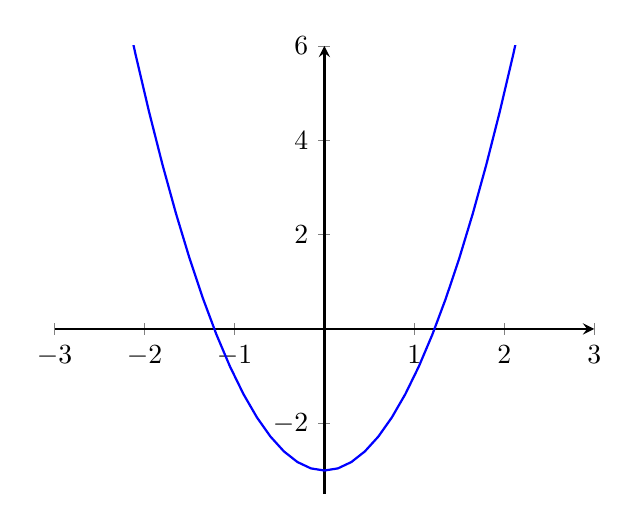
\begin{tikzpicture}
\begin{axis}[axis lines=middle
,samples=41, thick
,domain=-3:3, xmin=-3, xmax=3,
    ymin=-3.5, ymax=6,
    axis y line = middle
  ]

\addplot+ [no marks] {2 * x^2 - 3};
\end{axis}
\end{tikzpicture}
\caption{\label{fig:fctf}$f(x) = 2x^2 - 3$}
    \end{center}

  \end{figure}

  We use the
definition of convexity to formally show it. 
  Let $x, y \in \mathbb{R}$ and $\lambda \in [0,1]$. In order for $f(x)$ to be convex, it must satisfy the following condition:
	\[f(\lambda x + (1 - \lambda)y) \leq \lambda f(x) + (1-\lambda) f(y). \] 
We first write the inequation and use algebra to simplify it. 
\begin{align*}
	2(\lambda x + (1 - \lambda)y)^2 - 3  &\leq \lambda (2x^2 - 3)  + (1-\lambda) (2y^2 - 3) \\
	2\lambda^2 x^2 + 4\lambda(1 - \lambda)xy + 2(1-\lambda)^2 y^2 - 3 & \leq  2\lambda x^2 - 3\lambda + 2y^2 - 3  -2\lambda y^2 + 3\lambda\\
	2\lambda^2 x^2 + 4\lambda(1 - \lambda)xy + 2(1-\lambda)^2 y^2  &\leq 2\lambda x^2 + 2y^2 -2\lambda y^2 \\
	2\lambda^2 x^2 + 4\lambda(1 - \lambda)xy + 2y^2 -4\lambda y^2 + 2\lambda^2 y^2 & \leq 2\lambda x^2 + 2y^2 -2\lambda y^2 \\
	2\lambda^2 x^2 + 4\lambda(1 - \lambda)xy - 4\lambda y^2 + 2\lambda^2 y^2 & \leq 2\lambda x^2 -2\lambda y^2 \\
	2(\lambda^2 - \lambda) x^2 + 4\lambda(1 - \lambda)xy - 2\lambda y^2 + 2\lambda^2 y^2 & \leq  0 \\
	2(\lambda^2 - \lambda) (x^2 - 2xy + y^2) & \leq  0 \\
	2(\lambda^2 - \lambda) (x-y)^2  \leq  0.
\end{align*}

Since $\lambda \in [0,1]$, the quantity $(\lambda^2 - \lambda)$ is not
positive. As $(x-y)^2 \geq 0$, for any $x, y \in \mathbb{R}$, the final inequation is always true, which makes the starting inequation true as well. With this, we conclude that $f(x)$ is a convex function.

\item The function is plotted at Figure~\ref{fig:fctg}. It gives us
the intuition that the function is not convex, and not concave. We
show it. 


  \begin{figure}[htb]
    \begin{center}
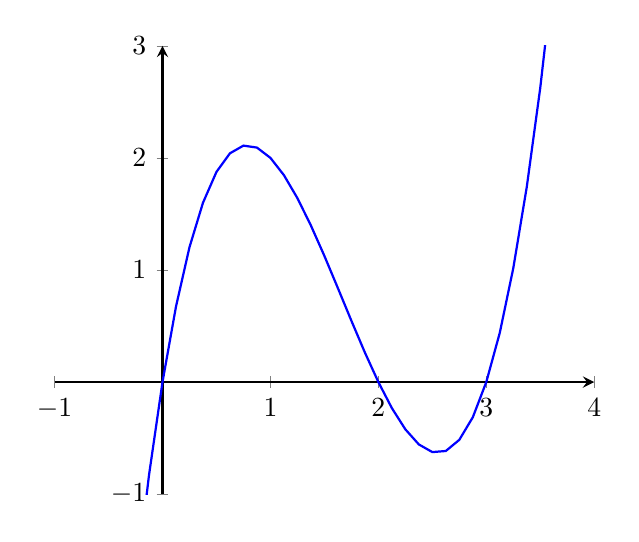
\begin{tikzpicture}
\begin{axis}[axis lines=middle
,samples=41, thick
,domain=-1:4, xmin=-1, xmax=4,
    ymin=-1, ymax=3,
    axis y line = middle
  ]

\addplot+ [no marks] {x^3 - 5 * x^2 + 6 * x};
\end{axis}
\end{tikzpicture}
\caption{\label{fig:fctg}$g(x) = x^3 - 5x^2 + 6x$}
    \end{center}

  \end{figure}



  In order for $g(x)$ to be convex, it must satisfy the following condition:
\[g(\lambda x + (1 - \lambda)y) \leq \lambda g(x) + (1-\lambda) g(y), \] 
for each $x, y \in \mathbb{R}$ and each $\lambda \in [0,1]$.

Similarly, in order for $g(x)$ to be concave, it must satisfy the following condition:
\[g(\lambda x + (1 - \lambda)y) \geq \lambda g(x) + (1-\lambda) g(y), \] 
for each $x, y \in \mathbb{R}$ and each $\lambda \in [0,1]$.

To show that the function is not convex, and not concave, we need to
prove the existence of $x$, $y$ and $\lambda$ that violate the above
inequalities. 
 Let us first rearrange the function in the following manner:
	\[g(x) = x^3 - 5x^2 + 6x = x (x-2) (x-3). \] 
From here, we see easily that $g(x) = 0$ for $x_1 = 0$, $x_2 = 2$, and $x_3 = 3$.

Let us further observe the function values in the points $x_1$, $x_2$, and $\lambda x_1 + (1-\lambda) x_2$, where $\lambda = 0.5$ for the sake of simplifying the proof:
\begin{align*}
g(x_1) = g(0) & = 0 \\
g(x_2) = g(2) & = 0 \\
g(\lambda x_1 + (1-\lambda) x_2) = g(1) & = 2 \\
\end{align*}
Since 
\[g(\lambda x_1+ (1 - \lambda)x_2) > \lambda g(x_1) + (1-\lambda) g(x_2),\] 
we can conclude that $g(x)$ is not convex.

Let us further observe the function values in the points $x_2$, $x_3$, and $\lambda x_2 + (1-\lambda) x_3$, where $\lambda = 0.5$, again for the sake of simplifying the proof:
\begin{align*}
g(x_2) = g(2) & = 0 \\
g(x_3) = g(3) & = 0 \\
g(\lambda x_2 + (1-\lambda) x_3) = g(2.5) & = -0.625 \\
\end{align*}
Since 
\[g(\lambda x_2+ (1 - \lambda)x_3) < \lambda g(x_2) + (1-\lambda) g(x_3),\] 
we can conclude that $g(x)$ is not concave either.

\end{enumerate}



